% !TeX spellcheck = en_US

\chapter{Design}
\label{chp:design}

	We have analyzed potential threats in the browser API and showed our results in the previous chapter. In this chapter, we present our design and implementation to proof that the results of our theoretical analysis are applicable in practical scenarios. 
	
	We designed our implementation as a set of components with different functionalities and privileges. This allows us to integrate some of our components into an existing, benign extension if the extension has declared the privileges needed to execute the component. As we do not change the extension's declared content and permissions, there will be no new warnings if the extension is updated. Especially Chrome disables an extension if the warnings shown on installation change with an update and the user has to explicitly accept the changes and subsequently re-enable the extension. 
	
	\autoref{fig:designOverview} shows a graphical overview of our design. The \textit{identification} and \textit{communication components} represent the core of our design and have to be included in the benign extension. Their duty is to collect as many pieces of information about the extension's current user as possible and send them to a remote server. If the server has successfully identified the user, we load the source code of our \textit{attack components} from the remote server and execute them. The implementation of the server and the identification algorithm is not in the scope of our work. 
	
	\begin{figure}[h]
		\centering
		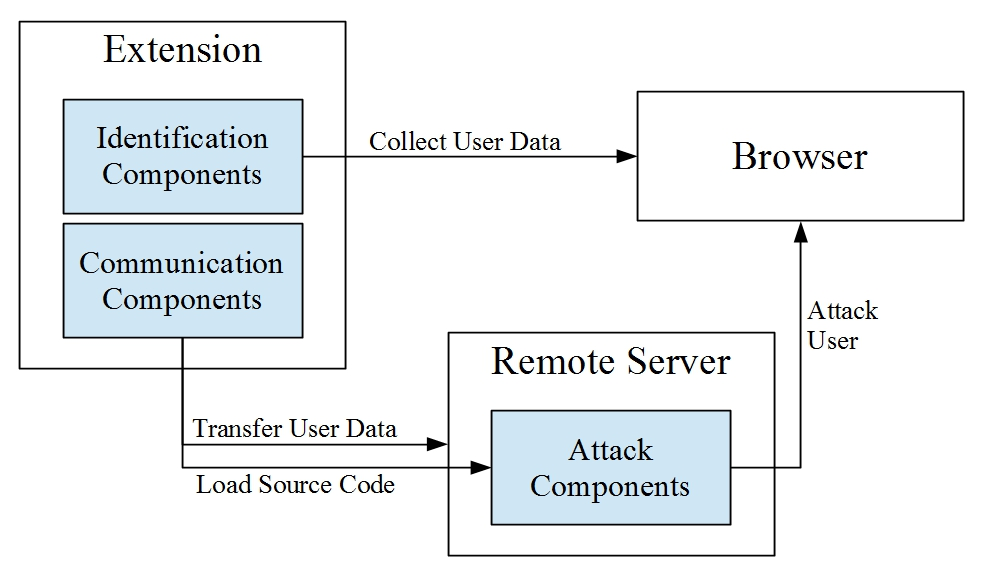
\includegraphics[width=0.7\textwidth]{./graphics/design_overview.png}
		\caption{Overview of our design.}
		\label{fig:designOverview}
	\end{figure}
	
	This design brings several advantages. As the bulk of our malicious implementations, namely the attack components, are not present at installation, a static analysis tool that uses content matching to find known malicious code pattern is less likely to detect our malicious intentions. Furthermore, the identification of the current user allows us not only to attack a worthwhile target but also to probably bypass a dynamic analysis. If we are able to detect that our implementation is currently the target of a dynamic analysis, we can fetch a benign script instead of our attack script. 

	We publish our implementations on a public git repository\footnote{\url{https://github.com/arnKo/Privacy-Threat-Analysis-Of-Browser-Extensions}}. In order to simplify the interaction with a web page's DOM, we use the popular web library \textit{jQuery}\footnote{\url{http://jquery.com/}}. 

\newpage	
\section{Identification}
\label{sec:identification} 

	Identifying the current user of our extension allows us to target our attack only to specific users. Beforehand, we can evaluate whether or not an attack is worthwhile if we collect as much as possible pieces of information about the user such his financial status or his position in a company we want to target. Furthermore, we are able to detect if our extension is target of an dynamic analysis such as the mentioned before \textit{Hulk} and \textit{WebEval} and evade detection by fetching a benign script instead of an attack component.
	
	In order to find approaches which we can use for our implementation, we first analyzed common methods to identify the current user of a web page and present them in this section. Then, we present our implemented components that collect information about the extension's current to later on identify him. We transfer collected information to our remote server which handles the identification. As the communication between the extension and a remote server is not part of this section, we refer to our implementations that we show in \autoref{sec:communication} as \textit{send method}.
	
\subsection{Common Methods}

	We have investigated common methods to identify the current user of a web page. In this section we present the techniques of user tracking and fingerprinting. 

	User tracking refers to the linking of multiple web pages that were visited by the same user. Applying this technique to web pages that belong to the same domain allows to follow the user's path through the domain's pages and determine his entry and exit points. This is commonly used for web analytics to help the website's author to improve the usability of his layout. User tracking between different domains produces an overview about the user's movement through the Internet. It is often used by advertising companies who extract the user's personal needs and preferences from the websites he visits to provide personalized advertisements.
		
	The general method for user tracking includes a unique identifier which is intentionally stored on the user's machine the first time he visits a tracking web page. If the identifier is retrieved on later occasions, it notifies the tracking party that the same user has accessed another web page. Several possibilities exists to store data inside the browser. We have listed some approach which we found in several research papers:
		
	\begin{itemize}
		\item \textbf{Tracking Cookies} A common used web technology to track users are HTTP cookies. If a user loads a web page any stored cookie from the same origin is send along the request. This simplifies the tracking, because the browser cares about the storage of the cookie and sends it automatically back to the server.
		
		\item \textbf{Local Shared Objects} Browser plugins use a technique similar to cookies to synchronize data between different browser sessions. The data is locally stored on the user's system. This allows to track the user behind different browsers. To store and retrieve an identifier inside a browser plugin, additional JavaScript is necessary.
		
		\item \textbf{Evercookie} This is a JavaScript framework implemented to produce persistent identifiers in a browser that are difficult to remove \cite{evercookie}. For that purpose, it uses multiple storage technologies such as HTTP and Flash cookies, HTML5 storages, web history and cache, and unusual techniques such as storing the identifier in RGB values of cached graphics. To hamper the removing from a browser, it recreates deleted identifiers as soon as the user visit a web site that uses the framework. The user has to delete every stored identifier to remove the evercookie completely. 
	\end{itemize}
	
	If a user loads a web page that includes a resource from a tracking third-party, any cookie that originates from the third-party's domain is send along the request that fetches the resource. This allows the third-party to track the user on every web page that includes their content. This kind of third-party content whose only purpose is user tracking is called a \texttt{Web Beacon}. A small image, commonly one pixel in size and transparent, is often used for that purpose. Because of its size it requires less traffic and its transparency hides it from the user. It is also used in HTML emails and acts as a read confirmation by notifying the sender that the email's content was loaded. Other nowadays more commonly used web beacons originate from social media such as Facebook's "like" button. 

	Previously described methods for tracking a user identify him based on some data which was intentionally stored on the user's system. Those stored identifiers are vulnerable to deletion by the user. A study from 2010 showed that a browser reveals many browser- and computer-specific information to web pages \cite{Eckersley:2010:UYW:1881151.1881152}. Collection and merging these pieces of information creates a fingerprint of the user machine. Creating a second fingerprint at a later point in time and comparing it to stored fingerprints allows to track and identify the user without the need to store an identifier on his computer in beforehand. As the same kind of information taken from different users will probably equal, it is necessary to collect as much information as possible to create a truly unique fingerprint. 
	
	The technique of fingerprinting is nowadays mostly used by advertising companies to get a more complete view of the user and his needs than from simple tracking and by anti-fraud systems that detect if the currently used credentials or device belong to the current user and are not stolen.

	There exists numerous scientific papers about fingerprinting from which we present a small subset of techniques with brief descriptions in the following list \cite{paulstone_historysniffing, MBYS11, Nikiforakis:2013:CME:2497621.2498133, Eckersley:2010:UYW:1881151.1881152, MS12, olejnik:hal-00747841}. 
	
	\begin{itemize}
		\item \textbf{Browser Fingerprinting} The browser provides a variety of technical information to a web page that can be used to generate a fingerprint of the currently used browser and machine. \autoref{tab:generalFingerprintingIncormation} shows examples of these properties and how to access them using JavaScript. 
		
		\begin{table}[h]
			\begin{tabular}{|l|l|p{0.47\textwidth}|} \hline
				\textbf{Property} & \textbf{JavaScript API} & \textbf{Example Output} \\ \hline
				System & \texttt{navigator.platform} & "Win32" \\ \hline
				Browser Name & \texttt{navigator.userAgent} & "Mozilla/5.0 (Windows NT 10.0; WOW64; rv:44.0) Gecko/20100101 Firefox/44.0" \\ \hline
				Browser Engine & \texttt{navigator.appName} & "Netscape" \\ \hline
				Screen Resolution & \texttt{screen.width} & 1366 (pixels) \\
				& \texttt{screen.height} & 768 (pixels) \\
				& \texttt{screen.pixelDepth} & 24 (byte per pixel) \\ \hline
				Timezone & \texttt{Date.getTimezoneOffset()} & -60 (equals UTC+1) \\ \hline
				Browser Language & \texttt{navigator.language} & "de" \\ \hline
				System Languages & \texttt{navigator.languages} & ["de", "en-US", "en"] \\ \hline
			\end{tabular}
			\caption{General fingerprinting information accessible through JavaScript and provided by the browser.}
			\label{tab:generalFingerprintingIncormation}
		\end{table}
		
		\item \textbf{Fonts} The fonts installed on the user's machine can serve as part of a user identification. The browser plugin \textit{Flash} provides an API that returns a list of fonts installed on the current system (\texttt{Font.enumerateFonts(true)})\cite{flashPlayerGetFonts}. If the Flash plugin is not available in a browser, JavaScript can be used to test whether particular fonts are available to the current web page or not. This approach needs a predefined list and may not cover unpopular fonts. It is implemented by writing a string with each font on the web page. If a font is not installed, the browser uses a fall-back font to draw the text. Comparing the width and height of the drawn font to those of the fall-back font gives an evidence whether or not the font is installed.
		
		\item \textbf{Canvas} Mowery er al. have notices that the same text drawn with the canvas interface results in a different binary representation on different computers and operating systems \cite{MS12}. They suppose the reasons for these different results are due to differences in graphical processing such as pixel smoothing, or anti-aliasing, differences in system fonts, API implementations or even the physical display. The basic flow of operations consists of drawing as many different letters as possible with the web page's canvas and executing the method \texttt{toDataURL} which returns a binary representation of the drawn image. 
		
		\item \textbf{History Sniffing} Reading out the user's web history can not only serve as fingerprinting method, but also to simplify user tracking. An outdated, but back then common approach to test if a user has visited a particular web page was to use the browser's feature to display links to already visited web pages in a different color. A JavaScript adds a list or predefined URLs to the web page's DOM as link elements and determines the displayed color. Nowadays, link elements that were queried by JavaScript calls behave like unvisited links which prevents this sniffing attack. A current approach detects the redrawing of link elements to determine if the underlying web page was visited before \cite{paulstone_historysniffing}. If a link is drawn the first time, it is drawn as an unvisited link and simultaneously a query to the browser's web history database is send. When the query returns the information that the web page behind the link was visited before, it redraws the link element. The time it takes to redraw the element can be captured with JavaScript giving the desired evidence.
		
		\item \textbf{JavaScript Benchmark Testing} The execution speed of a JavaScript engine depends on the implementation but also on the systems processor architecture and clock speed. Mowery et al. implemented a set of benchmark test suits to fingerprint different execution speeds \cite{MBYS11}. Using these information, they could distinguish between major browser versions, operating systems and micro architectures. 
	\end{itemize}	
 
\subsection{Implemented Components}
 
	We used the knowledge that we gained from investigation previously described methods to implement our components to collect user information. We implemented some components that execute and support user tracking or fingerprinting and present them in this section. These component collect technical information that can be used to identify the user's currently used device. Furthermore, we discovered that the currently displayed web page holds many pieces of personal user information that may help us to identify the person using the extension. For that purpose, we implemented several components that collect personal user information from particular websites and present them in this section, too. \autoref{tab:summaryUserIdentification} provides an overview of implemented components and their needed privileges.
  	
  	\begin{table}[h]
  		\centering
  		\begin{tabular}{|l|l|} \hline 
  			\textbf{User Identification Components} & \textbf{Needed Privileges} \\ \hline
  			Store identifier & \texttt{storage} \\ 	\hline
  			Web Beacon & content script \\ \hline
  			History Sniffing & \texttt{history} \\
  			& Content script \\	\hline
  			Bookmark Sniffing & \texttt{bookmarks} \\ \hline
  			Collect fingerprinting data & Content script \\ \hline
  			Additional fingerprinting data & \texttt{system.cpu} \\
  			& \texttt{system.memory} \\
  			& \texttt{management} \\ \hline
  			Read emails & Content script \\ 
  			Read facebook data & Content script \\
  			Read online banking data & Content script \\ \hline
  		\end{tabular}
  		\caption{Summary of implemented components to collect user information with needed privileges.}
  		\label{tab:summaryUserIdentification}
  	\end{table}
  
\subsubsection{Additional Fingerprinting Data} 
\label{sec:additionalFingerprintingData}

	The previously described techniques for fingerprinting can be executed from within a web page. Therefore, we can also execute them using a content script in an arbitrary web page. We implemented a component that collects fingerprinting values that the browser provides to a web page. Additionally, we can support this method by collecting technical information that the browser provides to an extension but not to a web page. These pieces of information help us to generate a more accurate fingerprint of the user's browser and system. In order to access the desired information, we need further permissions. \autoref{tab:fingerprintExtension} shows these pieces of information and the permissions needed to access them. 
	
	\begin{table}[h]
		\begin{tabular}{|l|l|l|} \hline
			\textbf{Permission} & \textbf{Information} & \textbf{Example} \\ \hline
			system.cpu & Number of processor kernels & \\
			& Processor's name & Intel(R) Core(TM) i5-3210M CPU @ 2.50GHz \\
			& Processor's capabilities & "sse", "sse2", "sse3"  \\ \hline
			system.memory & Memory capacity & 6501200096 \\ \hline
			management & List of installed extensions & Extension ID and version \\ \hline
		\end{tabular}
		\caption{Additional fingerprint information available to an extension.}
		\label{tab:fingerprintExtension}
	\end{table} 
	
\subsubsection{Web Beacon}
\label{sec:webBeacon}

	To allow user tracking between different websites, the website's developers have to explicitly include the Web Beacon into their web pages. For our design, we take use of the fact that we are able to access any web the user visits and can add new elements to its DOM. We implemented a component that uses only a content script in every web page. The script embeds an image in the web page which it fetches from our remote server. If our server sends a tracking cookie along the corresponding response, we are able to remotely track the user because our server gets notified every time the user loads a new web page.  

\subsubsection{Store Identifier In Extension}
\label{sec:storeIdentifier}

	If we have successfully identified the current user with other techniques, we store an unique identifier inside his instance of the extension. This simplifies his identification next time. An extension has its own local storage and Chrome even provides a cloud based storage which we use to store the identifier. In contrast to the web page's storage technologies such as cookies or the HTML5 local storage, the browsers Chrome, Opera, and Firefox do not provide a user interface to clear the extension storage. The user has to manually delete associated files on his hard drive. 
	
\subsubsection{History Sniffing}
\label{sec:historySniffing}

	The general method of history sniffing explicitly tests if a user has visited a particular web page. This strategy has the disadvantage that not all visited web pages are covered because a predefined list is necessary and often only contains popular web pages. To improve history sniffing, we use an extension to create a more complete list of the web pages that a user has visited and even capture additional information such as the time when and the order in which different web pages were visited. For that purpose, we can either use the \textit{history} module or a content script in every web page. Each approach has its advantages and disadvantages. 
	
	With a content script we can either execute the above described technique of history sniffing which uses a predefined list of web pages to explicit check, or store information such as the URL and the current time every time the content script is injected into a newly loaded web page. In \autoref{sec:webBeacon}, we have already presented a component that exactly executes this task. Our implementation of a Web Beacon notifies us every time the user has opened a new web page by fetching a resource from our remote server. To get the URL of the visited web page, we can simply transfer it as parameter in the web request that fetches the resource. The disadvantage of using a content script for history sniffing is, that we can not retrieve visited web pages from before the extension's installation or while the extension is disabled. Therefore, it is not an ideal fingerprinting technique because it has to be active for some time to be effective. However, it is a simple alternative if the \textit{history} module is not available because the extension does not have the corresponding permission.
	
	Using the history module allows us to retrieve all visited web pages at once. It provides two for us useful methods \texttt{search} and \texttt{getVisits}. The first method allows us to retrieve the URLs of all web pages the user has visited and the second one gives us detailed information about every time the user has visited a particular URL such as the concrete time, the referring web page, and how the user has entered the web page. In comparison to using a content script, the history module gives us more pieces of information and executes at once. However, the browser's history is vulnerable to deletion or disabling by the user and is disabled if the user uses an incognito window.
	
	We implemented a component that executes a history sniffing attack using the history module. It queries for all visited web pages that the browser has stored and retrieves information about every time the user has visited each. The method that returns all web pages takes as arguments a start and end date that limit the returned list to visited web pages in the given time interval and the maximum number of returned entries. We set the start date to zero because it defaults to 24 hours in the past and the number of returned values to the maximum possible value. This returns us the complete list of stored entries.
	
\subsubsection{Bookmark Sniffing}
\label{sec:bookmarkSniffing}

	Similar to history sniffing, we retrieve the user's bookmarks as additional information for a fingerprint but also to get information about his preferred web pages. This allows us to explicit target web pages with our attacks that the user is high likely to visit. Our implemented component needs the \textit{bookmarks} permission to access the corresponding module. The browser stores the bookmarks in a tree structure. Our component uses a recursive function to traverse the tree and extract the bookmarks title and URL. In every recursion step we check if the current node contains a title and an URL. If this is not the case, the current node is not a bookmark but a folder.

\subsubsection{Personal User Information}
\label{sec:personalUserInformation}
	
	Besides the before described techniques of user tracking and fingerprinting, an extension has more efficient ways to identify a user. The extension has full access to any web page that the user visits and is able to read out any information that is stored inside these pages. It allows us to even identify the person behind the web user by collection personal information such as his full name, address, or phone number. 
	
	While developing the components that extract personal user data, we faced several challenges. First at all, an extension whose purpose is to obtain particular data from a web page retrieves the targeted values directly from the web page's DOM and thus heavily depends on the DOM's structure. Due to strong differences between the structures of different web applications, we did not implement a general approach that collects the targeted information from multiple applications, but instead target specific web applications. 
	
	Secondly, many modern web pages are of a dynamic nature. They load additional content while the user navigates the page. In order to be able to collect information that are fetched dynamically, we periodically query the web page and extract desired values. Another challenge that we faced were JavaScript driven text editors in separate iframes. To extract their content, we programmatically injected a small content script in all frames of the current web page. The script evaluates if it is active in the targeted iframe, collects the desired content, and returns it. 
	
	We have extracted three categories of web applications as worthwhile targets to collect user data:
	\begin{itemize}
		\item \textbf{Social Media} Many people use real names and other personal information for their social media account. If the user visits his account, we can read out his personal data. Furthermore, we can extract information such as the user's social or business environment while the user visits the social web pages of other people he interacts with. \\
		We implemented a component that collects the user's personal information while he navigates through his Facebook account. Our component retrieves the user's name, the URL of his main page, the names of his friends, locations that he has shared with Facebook, and other personal information from his main page such as his date of birth, home town, or gender.
		
		\item \textbf{Online Banking} We can identify the current user based on his account numbers if he uses his online banking account. Moreover, we can extract his financial status which gives us information whether or not an attack on his finances is worthwhile. \\
		We implemented a component that targets a specific online banking platform. It iterates the user's banking accounts and selects the account's name, identification number, and current balance.
		
		\item \textbf{Email Account} If the user sends and receives emails on his online email account, we can read those and collect probably valuable information that he shares with his acquaintance or other people. \\
		We implemented two components that target a specific online email client. The first one reads the user's outgoing emails. For that purpose, it registers a listener to the "email send" button and then collects all recipients and the emails body when the user sends the mail. The second component retrieves the emails in the user's inbox. It awaits that the user opens a received email and extracts the sender and body.
	\end{itemize}
	
\clearpage
\section{Communication}
\label{sec:communication}

	In the previous section, we have shown our implementations to collect information about the current user to identify him. We need to transfer these data to a remote server which is in charge of the identification. Furthermore, if the identification was successful, we want to attack the user by loading the source code for some malicious behavior from the server. In this section, we present different approaches to transfer information between the extension and a remote server and to fetch the source code for explicit attacks. \autoref{tab:summaryRemoteCommunication} and \autoref{tab:summaryFetchScript} provide an overview of implemented components for sending data to a server and remotely fetching scripts with needed privileges.
	
	\begin{table}[h]
		\centering
		\begin{tabular}{|l|l|} \hline
			\textbf{Remote Communication Components} & \textbf{Needed Privileges} \\ \hline
			XMLHttpRequest & \texttt{http://*/*, https://*/*}  \\
			Iframe & Content script \\	
			\hline
		\end{tabular}
		\caption{Summary of implemented communication components with needed privileges.}
		\label{tab:summaryRemoteCommunication}
	\end{table}
	
	\begin{table}[h]
		\centering
		\begin{tabular}{|l|l|} \hline
			\textbf{Remote Script Fetching Components} & \textbf{Needed Privileges} \\ \hline
			Script element in background & Modified CSP with remote server URL \\
			Script element in content script & Content script \\
			XMLHttpRequest, execute in background & \texttt{http://*/*, https://*/*}, modified CSP with \texttt{unsafe\_eval} \\
			XMLHttpRequest, execute in content script & \texttt{http://*/*, https://*/*}  \\
			Mutual extension communication & Content script, second extension \\ 
			\hline
		\end{tabular}
		\caption{Summary of implemented components to load and execute a remote script with needed privileges.}
		\label{tab:summaryFetchScript}
	\end{table}
	
\subsection{Remote Communication Components}
\label{sec:remoteCommunication}

	We often come to a point where we have to transfer information from the active extension to a remote server or vice versa. For example, if we want to transfer collected information for identification or stolen personal user data or we want to give the extension the command to execute an attack. We implemented several, partly interchangeable components for that purpose and present them in this section.

\subsubsection{XMLHttpRequest}
\label{sec:xhrCommunication}

	Extensions are able to make a web request to a remote server with a XMLHttpRequest. If called from within a web page, the XMLHttpRequest will be blocked by the Same Origin Policy if the target does not match the page's origin. However, the same restriction does not apply to extensions. It is only restricted by the declared host permission in its manifest. For this component, the extension needs a host permission that matches any URL such as \texttt{http://*/*}, \texttt{https://*/*}, or \texttt{<all\_urls>}. 

\subsubsection{Iframe}
\label{sec:iframeCommunication}

	Another strategy that we use to transfer information to a remote host uses the mechanics of an \textit{iframe} element. Its task is to display a web page within another web page. The displayed web page is defined by the URL stored inside the iframe's \texttt{src} attribute. If the URL changes, the iframe tries to load the web page by sending a request to the defined URL. Adding parameters to the URL allows to send data to the targeted server. This strategy was previously described by Liu et al. \cite{Liu12chromeextensions:}.

	The Same Origin Policy creates a boundary between the iframe and its parent web page. It prevents scripts to access content that has another origin than the script itself. Therefore, if the web page inside the iframe was loaded from another origin than the parent web page, the iframe's JavaScript can not access the parent web page and vice versa. The same restriction applies to contents script, too. However, an extension can execute another content script in the iframe's web page to access its content. For that purpose, it has to enable the \texttt{all\_frames} option for a content script either statically in the manifest or for a programmatically injection. We use this fact for our component and use it as a two way communication channel. Executing a second content script inside the iframe, allows us to read information that a server has embedded inside the fetched web page.

\subsection{Remote Script Fetching Components}
	
	As our implementation relies on fetching the source code for a particular attack from a remote server, we present our implemented components in this section. Fetching a script remotely from a server is also some kind of communication. Therefore, some components that we present in this section use similar approaches like earlier presented components for communication in \autoref{sec:remoteCommunication}. 
	
\subsubsection{Script Element In Background}
\label{sec:scriptElementInBackground}
	
	HTML pages which are bundled in the extension's installation, can include script elements with a source attribute pointing to a remote server. If the extension is executed and the page is loaded, the browser automatically loads and executes the remote script. This mechanism is often used to include public scripts, e.g. from Google Analytics. 
	
	An extension needs to explicitly state that it wants to fetch remote scripts in its background page. The default Content Security Policy disables the loading of scripts per script element which have another origin than the extension's installation. We can relax the default CSP and enable the loading of remote scripts over HTTPS by adding a URL pattern for the desired origin. 
	
\subsubsection{Script Element In Content Script}
\label{sec:scriptElementInContentScript}

	If we want to execute a remote loaded script only in the scope of a web page, we can take use of the DOM API. It allows us to add a new script element to the current web page. If we set the source attribute of the script element to the URL of a remote server, the browser will fetch and execute the script. Our component that executes this strategy does not need additional permissions besides a single content script in the targeted web page. 
	
\subsubsection{XMLHttpRequest}
\label{sec:xhrFetching}

	In \autoref{sec:xhrCommunication} we have demonstrated that an extension can execute a web request to a remote server with the XMLHttpRequest API. To execute the request, our component needs host permissions to any origin. This approach allows us not only to transfer information to a remote server, but also to receive any data, especially the source code for the attack components. We receive the source code in text form and have to forward it to the browser's JavaScript interpreter to execute it.
	
	Before we can execute a remote loaded script, we have to consider what the scripts objectives are. Whether it should act in the extension's background or as a content script. If the first case applies, we can use the JavaScript method \texttt{eval} to execute the remote loaded code as a JavaScript application. The use of eval is frowned upon because it is a main source of XSS attacks if not used correctly \cite{mozillaDangerousEval}. On that account, the default Content Security Policy disables the use of eval in the extension's background process. We can relax the default policy and add the key \texttt{unsafe\_eval} to lift the restriction.
	
	If we want to execute the remote loaded script as a content script, we can programmatically inject it. The method \texttt{chrome.tabs.executeScript} executes a given string as a content script in a currently open tab. The use of this function is not restricted by a permission. However, to access the web page in the tab, the extension needs a proper host permission that matches the web page's URL. As we have fetched the script with an XHR, we have already declared host permissions that match any URL to execute the request.
	
\subsubsection{Mutual Extension Communication}
\label{sec:mutalExtensionCommunication}

	An extension is able to communicate with another extension. This opens the possibility of a permission escalation as previously described by Bauer et al. \cite{extensions:cns14}. The extension which executes the attack does not need the permissions to fetch the malicious script. Another extension can execute this task and then send the remote script to the executing extension. This allows to give both extensions less permissions and thus making them less suspicious especially for automatic analysis tools. To detect the combined malicious behavior, an analysis tool has to execute both extensions simultaneously. This is a very unconventional approach, because an analysis often targets only a single extension at a time. 
	
	A communication channel that does not require any special interface, can be established over any web page's DOM. All extensions with an active content script in the same web page have access to the same DOM. The extensions which want to communicate with each other can agree upon a specific DOM element and set its text to exchange messages. Another way to exchange messages is to use the DOM method \texttt{window.postMessage}. This method dispatches a \texttt{message} event on the web pages \texttt{window} object. Any script with access to the web page's \texttt{window} object can register to be notified if the event was dispatched and then read the message. 
	
	We implemented two components that execute the described strategy. The first one dispatches a message on the window object of the current web page and the second registers for the message event and reads the attached message. We admit that these components will have almost no scope for application, because a user needs to have two malicious extension installed for this strategy to work. It serves, therefore, more as an example to show possible attack vectors.


\clearpage
\section{Execution}
\label{sec:execution}

	We have already shown how we collect information to identify the current user, transfer it to the remote server that is in charge to evaluate the data, and how we fetch the source code of an attack in the case that the identification was successful. In this section we finally present our concrete attack implementations. For that purpose, we present known attack scenarios that make use of an extension's capabilities followed by a presentation of our implemented attack components. \autoref{tab:summaryAttacks} provides an overview of implemented attack components and their needed privileges.
	
	\begin{table}[h]
		\begin{tabular}{|l|l|} \hline 
			\textbf{Attack Component} & \textbf{Needed Privileges} \\ \hline
			Steal sensitive user data & Content script \\ \hline
			Steal form data & Content script \\ \hline
			Steal credentials & Content script \\ \hline
			Manipulate form values & Content script \\ \hline
			Manipulate form target URL & Content script \\ \hline
			Manipulate link target URL & Content script \\ \hline
			Redirect request & \texttt{http://*/*, https://*/*, webRequest, webRequestBlocking} \\ \hline
			Execute concealed attack in iframe & Content script \\ \hline
			Execute concealed attack in inactive tab & \texttt{http://*/*, https://*/*, tabs} \\ \hline
			Execute concealed attack in background window & \texttt{http://*/*, https://*/*} \\ \hline
			Denial of Service & Content script \\ \hline
			Download and open file & \texttt{downloads, downloads.open, downloads.shelf} \\ \hline
			Exchange a downloaded file & \texttt{downloads} \\ \hline
			Exchange a currently downloading file & \texttt{downloads} \\ \hline
			Steal cookies from current web page & Content script \\ \hline
			Steal all cookies & \texttt{http://*/*, https://*/*, cookies} \\ \hline
			Disable another extension & \texttt{management} \\ \hline
			Remove request response header & \texttt{http://*/*, https://*/*, webRequest, webRequestBlocking} \\ \hline
		\end{tabular}
		\caption{Summary of implemented attack components with needed privileges.}
		\label{tab:summaryAttacks}
	\end{table}
	
\subsection{Attack Scenarios}

	In this section we present two attack scenarios that an extension facilitates. The \textit{Man-in-the-browser} attack manipulates web requests and often targets the user's online banking account. This allows an attacker to manipulate a transaction's target or amount. Contrary, a \textit{botnet} of browser extensions allows to execute wide scaled web attacks such as spamming or DDoS attacks. The extension's current user is often not the target of an attack but his device is misused to execute attacks against others.

\subsubsection{Man in the Browser}
	
	The Man-in-the-browser (MITB) is a browser based attack related to man-in-the-middle attack (MITM) \cite{Curran:2012:MBA:2433195.2433198}. The MITM is an attack scenario in computer cryptography against the communication between two parties who directly communicate with each other. The attacker secretly either intercepts and alters the traffic or he impersonates one party and deceives the other party who still thinks he communicates with the impersonated party. MITM has to bypass security layers such as encryption or mutual authentication to gain access to the communication channel. The attacker uses either vulnerabilities in obsolete cryptography algorithm or exploits in buggy implemented soft- or hardware. An MITB attack is located inside the browser from where it intercepts in- and outgoing web requests. The attack will be successful irrespective of security mechanisms because it takes place before any encryption or authentication is applied. 
	
	An MITB attack often aims to manipulate the traffic between the user and a trusted third party. A common target of an MITB attack is an online banking portal. An attack my look like the following example. The user logs into his account at the targeted banking website. He initiates a transaction and sends the data to the bank's server. The MITB code reads the outgoing request and changes the target account or the transfer amount. The bank's sever is not able to recognize the manipulated request because it receives the information with a valid authentication from the user. It executes the transfer and sends back a receipt. The MITB code reads the response's HTML code and changes the manipulated data back to its original state. To mitigate these attacks, modern banking systems use further security features such as a TAN generator that calculates an additional token from the targeted account's identification number, the transaction amount, and some secrete stored inside the user's banking card. Even if the MITB attack would know the calculation for the token, he has no access to the externally stored secret.
	 
	An MITB often comes in the form of a Trojan Horse that infects the browser with its code. An extension facilitates this attack, because it has full access to the displayed web pages and can modify web requests. 
	
\subsubsection{Botnet}

	A botnet is a network consisting of multiple compromised clients that can be controlled to execute large scaled web attacks such as Distributed Denial of Service (DDoS) or spamming attacks. DDoS is a web based attack targeted to make an web service unavailable by overwhelming it with requests. A botnet can be used to call the web service from different sources multiple times per second. The attack either targets the network and flood its bandwidth or the application itself using up the computer's resources. This results in the web service being unavailable for the general public. \cite{liu2011botnet}
	
	Browser extensions in a botnet were previously researched by Liu et al. \cite{liu2011botnet}. As a proof-of-concept, they developed two extension that act as bots, one for Chrome and one for Internet Explorer. Their extension's can execute DDoS attacks, email spamming, and steal the user's credentials. To send an email, the extension uses the user's email account. If the user logs into his account, the extension executes a web request to send an email with the spamming content. The email server will actually execute the request because the user's credentials are send along. 
	
	A botnet needs a communication channel that allows the attacker to control the bots. For their extensions, the researchers use the automatic update and modify the content of a configuration file. The extension reads the file and acts accordingly. After the attacker publishes a new update, which will start a new attack, the update will be installed as soon as the browser is active. As the installation of the update is distributed in time, the attack is, too. This hampers the detection of the botnet because not all attacks are executed simultaneously.
	
\subsection{Implemented Components}
	
	We investigated known attack scenarios that are executable using an extension and use the gained knowledge to implement several attack components. In this section we present these components which our communication components will fetch from a remote server after a successful identification of the current user. Depending on how we have fetched the attack's source code, we need different permissions to execute the attack. In the case that the attack is executed in the scope of a web page, we need either an already active content script that executes the attack or host permissions to inject the attack as independent content script into the web page.

	In \autoref{sec:identification}, we have already shown that we are able to obtain personal user information by extraction them from the web pages that the user visits. Previously, we collected these information to generate a fingerprint of the current user and identify him based on this fingerprint. Of course, if we have already obtained sensitive information, we are able to misuse them and harm the user. Therefore, we also use the components presented in \autoref{sec:identification} as attack components to steal sensitive user data.

\subsubsection{Accessing Form Data}
\label{sec:stealFormData}

	The user often transmits sensitive information to a web server using a web form. We can intercept and steal these transmitted data using the simple code snippet \lstinline|$('form').submit(function() { send($(this).serialize()); })|. The \textit{jQuery} library allows us to simply register an event on each form elements of the current web page that is dispatched, if the form is submitted by the user. In this case, we again use jQuery to serialize the form's content and forward it to our send method. This attack is a very general approach that targets any form element in all web pages.
	
	We find a more concrete application for the previously described attack on authentication web pages. These usually contain a web form in which the user enters his credentials to authenticate against a web application. If we obtain his credentials, we can impersonate the user on this particular application. Our implementation for this attack is very similar to the previously described attack. To explicitly target only authentication forms, we search for an input filed of type password on the page. These are typical components of a web form in combination with a text field in which the user enters his username. If we have found one, we select the corresponding form element and attach again an event handler that is triggered if the user submits the form. The event handler will then read out the form's values.

	The browser provides a storage for entered credentials to the user. If the user has stored his credentials for a particular web page and opens this page on a later occasion, the browser will fill in the stored credentials. We implemented another component that steals the credentials from an authentication form after the browser has filled in the desired values. Again, we use a similar implementation than the before described attack. We first search for an input element of type password to identify the authentication form. Afterwards, we use the function \texttt{setTimeout} and wait for 500 milliseconds to give the password manager the time to fill in the credentials. Finally, we extract the desired values and send them to our remote server.
		
\subsubsection{Manipulate Web Requests}
\label{sec:manipulateWebRequests}

	An extension is able to manipulate any outgoing web request. We can redirect a GET request to load a malicious lookalike of the original web page, redirect a POST request to obtain probably sensitive values, or manipulate the values of a request's body to harm the user. The user initiates most requests from within a web page. Therefore, we use a content script to manipulate URLs and form values inside a particular web page. Additionally, we use the \texttt{webRequest} module to intercept and manipulate outgoing web requests.
	
	We implemented a component that manipulates the value of a form field with this code snippet. For this attack, we need explicit knowledge about the targeted web page's structure. We need a CSS selector to find the targeted form and a CSS selector to find the form's targeted value. This attack may be used to change the transaction amount if the user uses his online banking account for a transaction or change the transaction's target. 

	We can change the target to which the values of a form are transmitted by manipulating the forms \texttt{action} attribute. For that purpose, we use the following code snippet: \lstinline|$('form').attr('action', MALICIOUS_URL);|. First, we select a form element and set its action attribute to the URL of a malicious web page. Similar, we can change the targeted web page of a link element. Again, we us a small code snippet: \lstinline|$('a[href~=' + TARGETED_URL + ']').attr('href', TARGET_URL);|. This time, we select a link element whose current URL targets a particular web page and set its \texttt{href} attribute to the URL of a malicious web page. We implemented an equal attack which uses the \texttt{webRequst} module instead of a content script. This allows us to redirect any web request. To execute this attack, the extension needs the \texttt{webRequest} and \texttt{webRequestBlocking} permissions and proper host permissions for the targeted web page such as \texttt{http://*/*} and \texttt{https://*/*}. 
	
\subsubsection{Execute Attack In a Background}
\label{sec:executeAttackInBackground}

	We implemented several components that open predefined web pages to execute particular attacks such as to steal possibly stored credentials from the browser's password manager. Different strategies to hide the loading of a new web page were previously discussed by Bauer et al. \cite{extensions:cns14}. We implemented three described approaches:
	
	\begin{enumerate}
		\item Load the targeted web page in an invisible iframe inside any web page.
		\item Load the targeted web page in an inactive tab and switch back to the original web page after the attack has finished.
		\item Open a new tab in an inactive browser window and load the targeted web page in this tab. Close the tab after the attack has finished.
	\end{enumerate} 
	
	The first approach is the least reliable one. There exists several methods to enforce that a web page is not displayed in an iframe. The standardized approach is to use the \texttt{X-Frame-Option} HTTP header which is compatible with all current browsers \cite{xFrameOptionsSpezification, xFrameOptionsCompability}. This transfers the responsibility to enforce that the web page is not loaded into an iframe to the browser. Other approaches use JavaScript to deny the web page's functionality if it is loaded in an iframe or to move the web page's content from the iframe to the main frame.
		
	In order to open a particular web page in an iframe, we use a content script with the \texttt{any\_frame} option which enables the execution of the content script in all sub-frames of the current web page such as iframes.Our implementation consists of two steps. First, we check if the content script is currently active in the window's main frame with the conditional statement \lstinline|window.self === window.top|. In this case, we send a message to the extension's background to retrieve the URL or a targeted web page. This is necessary because the content script itself can not store data - in our case a list of targeted URLs - between different instances of itself. Next, we create a new iframe element, turn it invisible for the user, attach it to the current web page, and load the targeted web page. Because we set the \texttt{any\_frame} option, the browser will execute our content script in the newly loaded web page. The check if we the script is currently active in the main frame will fail and we can execute the second part of our script which executes another component to attack the loaded web page.
	
	The second and third approach work very similar. Both use the browser's tab system to open a particular web page. Therefore, the components needs the \texttt{http://*/*} and \texttt{https://*/*} host permissions and for the second approach additionally the \texttt{tabs} permission.
	
	In order to open a particular web page in an inactive tab, we use the browser's tab system provided through the \texttt{tabs} module. First, we search for an inactive tab using \lstinline|chrome.tabs.query({active: false});|. We store the URL of the tab's current web page, to later switch it back. To access the web page's URL, we need the \texttt{tabs} permission. Afterwards, we load the targeted web page into the tab and inject a content script that executes a particular attack. The content script will send a message to the extension's background to indicate that it has finished executing the attack. If we receive this message, we will load the tab's original web page into the tab to disguise our attack.
	
	In order to open a particular web page in a background window, we use a similar implementation to the before described approach to load the web page into an inactive tab. For this approach, we do not search for an inactive tab instead we search for a tab that is not in the current browser window using \lstinline|chrome.tabs.query({currentWindow: false});|. We also do not need the \texttt{tabs} permission, because we do not access the URL of the tab. Instead, we extract the tab's window id and open a new tab inside the same window using \lstinline|chrome.tabs.create({url: TARGET_URL, windowId: windowId});|. Simultaneously, we load the targeted web page into the newly created tab. Now we can execute our attack in the tab and close it when the attack has finished.
	
	We tested our implementations in Chrome, Opera, and Firefox with our attack implementation to steal possibly stored credentials from the browser's password manager which we have described in \autoref{sec:stealFormData}. We discovered that the attack is only successful in Firefox. The reason that the attack does not work in Chrome and Opera is that JavaScript has no access to the value of a password input field before any user interaction with the web page occurred. This is an intended security feature to prevent exactly this kind of attack \cite{chromiumBlogPasswordInput}.


\subsubsection{Denial Of Service}
\label{sec:DoS}
	
	An extension can execute unrestricted web requests from within a content script using an iframe element. We use this fact to implement a component that executes a Denial of Service attack. Our component uses a single content script that repeatedly creates a new iframe element and loads the targeted web page. To prevent that the browser fetches the web page from its cache, we add a random number as parameter to the target URL. This attack is especially effective if the extension is active in multiple browsers. We can send the command to execute the attack to all active extensions, using a communication technique that we have described in \autoref{sec:communication}.

\subsubsection{Download Harmful Files}
\label{sec:downloads}

	Using the \textit{download} module, an extension is able to monitor and cancel the user's downloads or to initiate a download itself and even to open a downloaded file. We misuse this feature to get access to the user's machine which the extension itself does not have. For that purpose, we implemented a component that automatically downloads and opes a file which can contain a malware.
	
	We implemented a component that downloads a file and opens it. For that purpose, the extension needs the \texttt{downloads} permission and additionally the \texttt{downloads.open} permission to open the downloaded file and the \texttt{downloads.shelf} permission to hide the download from the user. The \texttt{downloads.shelf} permission enables an extension to show or remove the shelf at the bottom of the browser that shows active downloads. \\
	To open a downloaded file, the user has to interact with the extension and deliver some kind of input such as a mouse click. If no user input is given, the browser blocks the opening of a file. For our implementation, we use a content script that adds an on click event to each element of the current web page. If the user clicks any element, we send a message to our background script which also transfers the desired user input and use this to open the file. \\
	We start our component by disabling the download status bar of the browser so that the user does not see the download. Then, we initiate the download of a harmful file. When the download is finished, we await a message from our content script and use the transmitted mouse click to open the downloaded file. Finally, we delete our file from the browser's list of downloads and re-enable the download status bar to prevent that the user notices the download.
	
	We implemented another component that cancels a download which the user has initiated and then initiate a download ourself of a harmful file. Our goal is that the user does not notices that we cancel his download and initiate a second one and then opens the harmful file. For that purpose, we extract the name and mime-type of the file that the user wants to download and send it along the request to download the harmful file. This allows us to set the mime-type and filename of the harmful file. To further hide our attack, we may deactivate the status bar while we exchange the downloads if the extension has the \texttt{downloads.shelf} permission. \\

\subsubsection{Steal Cookies}
\label{sec:stealCookies}

	We implemented two components for our design, that follow different strategies to steal currently stored cookies from the user's browser. Cookies often contain a session id that authenticates the current user to a web application. If we obtain this information, we are able to impersonate the user on this particular web application. 
	
	JavaScript in a displayed web page has access to cookies that belong to the same domain as the web page with exception to cookies with the \texttt{httpOnly} key set. We use this in our first implementation that uses a single content script in any web page. The cookies are stored inside the DOM and we access them with with \texttt{document.cookie}. Obviously, this implementation is restricted to web page's that the user visits while the extension is active and without access to \texttt{httpOnly} cookies. Therefore, we implemented the second approach that uses the \texttt{cookies} module. Using this module, we have access to all cookies that are currently stored inside the browser without restrictions besides the extension's permissions. To use it, the extension needs the \texttt{cookies} permission and host permissions for any web page such as \texttt{http://*/*} and \texttt{https://*/*}. We use the method \lstinline|{chrome.cookies.getAll| which accepts an object to filter retrieved cookies based on the cookie's values such as the URL, domain, or its secured state.

\subsubsection{Disable Other Extension}
\label{sec:disableOtherExtension}

	In order that other, security relevant extensions do not block our attack implementations, we implemented a component that disables another extension. For that purpose, the extension needs the \texttt{management} permission which gives access to the correspondent module. To disable another extension, we need the targeted extension's name or id.
	The method \lstinline|chrome.management.getAll| returns a list of currently installed extensions. We iterate the list and compare the name or id of each extension to determine the targeted one. If we find the matching extension, we use the method \lstinline|chrome.management.setEnabled| to deactivate it.

\subsubsection{Remove Security Headers}
\label{sec:removeSecurityHeaders}
	
	We implemented a component that removes security relevant response headers. We use this implementation to support our component that opens a particular web page in an iframe which we have shown in \autoref{sec:executeAttackInBackground}. This attack is hampered by web pages that use the \texttt{X-Frame-Option} header, because the browser disallows displaying the web page inside an iframe. By removing this header from the web request's response, we improve the attacks' success rate. Similar, we can support any content script that executes web requests to fetch content. If the web page uses a Content Security Policy that blocks the loading of scripts or other web pages, we can remove the CSP and allow our content script to execute its task.
	
	Our component needs the \texttt{webRequest} permission to access the corresponding module and the \texttt{webRequestBlocking} permission to be able to intercept the request's processing until we have removed the targeted response header. Additionally, the component needs host permissions that match the request's target URL. 